
\chapter{Point de Situation}
\label{chap:choix}

\section{Contexte}


\section{Rappel de notre projet}

Suite à notre état de l'art, nous avons décidé de réaliser notre système de détection en installant un maillage de capteur qui se baseront sur le système du Montréal 3V2. Chaque capteur sera connecté à un \rpi 2 \footnote{La documentation technique du Raspberry PI est situé en annexe à la page \pageref{annexe:rpi}}. De plus, chaque \rpi communiquera avec un ordinateur central qui traitera les données pour les afficher sur une interface graphique. Les données qui seront transmises sont: le numéro du \rpi, la position du capteur, et le gisement du drone par rapport au capteur. Enfin, l'ordinateur central communiquera avec une application android qui notifiera le client de la présence d'un drone comme on peut le voir sur la figure \ref{fig:inst}.
~\\

\begin{figure}[!h]
  \centering
  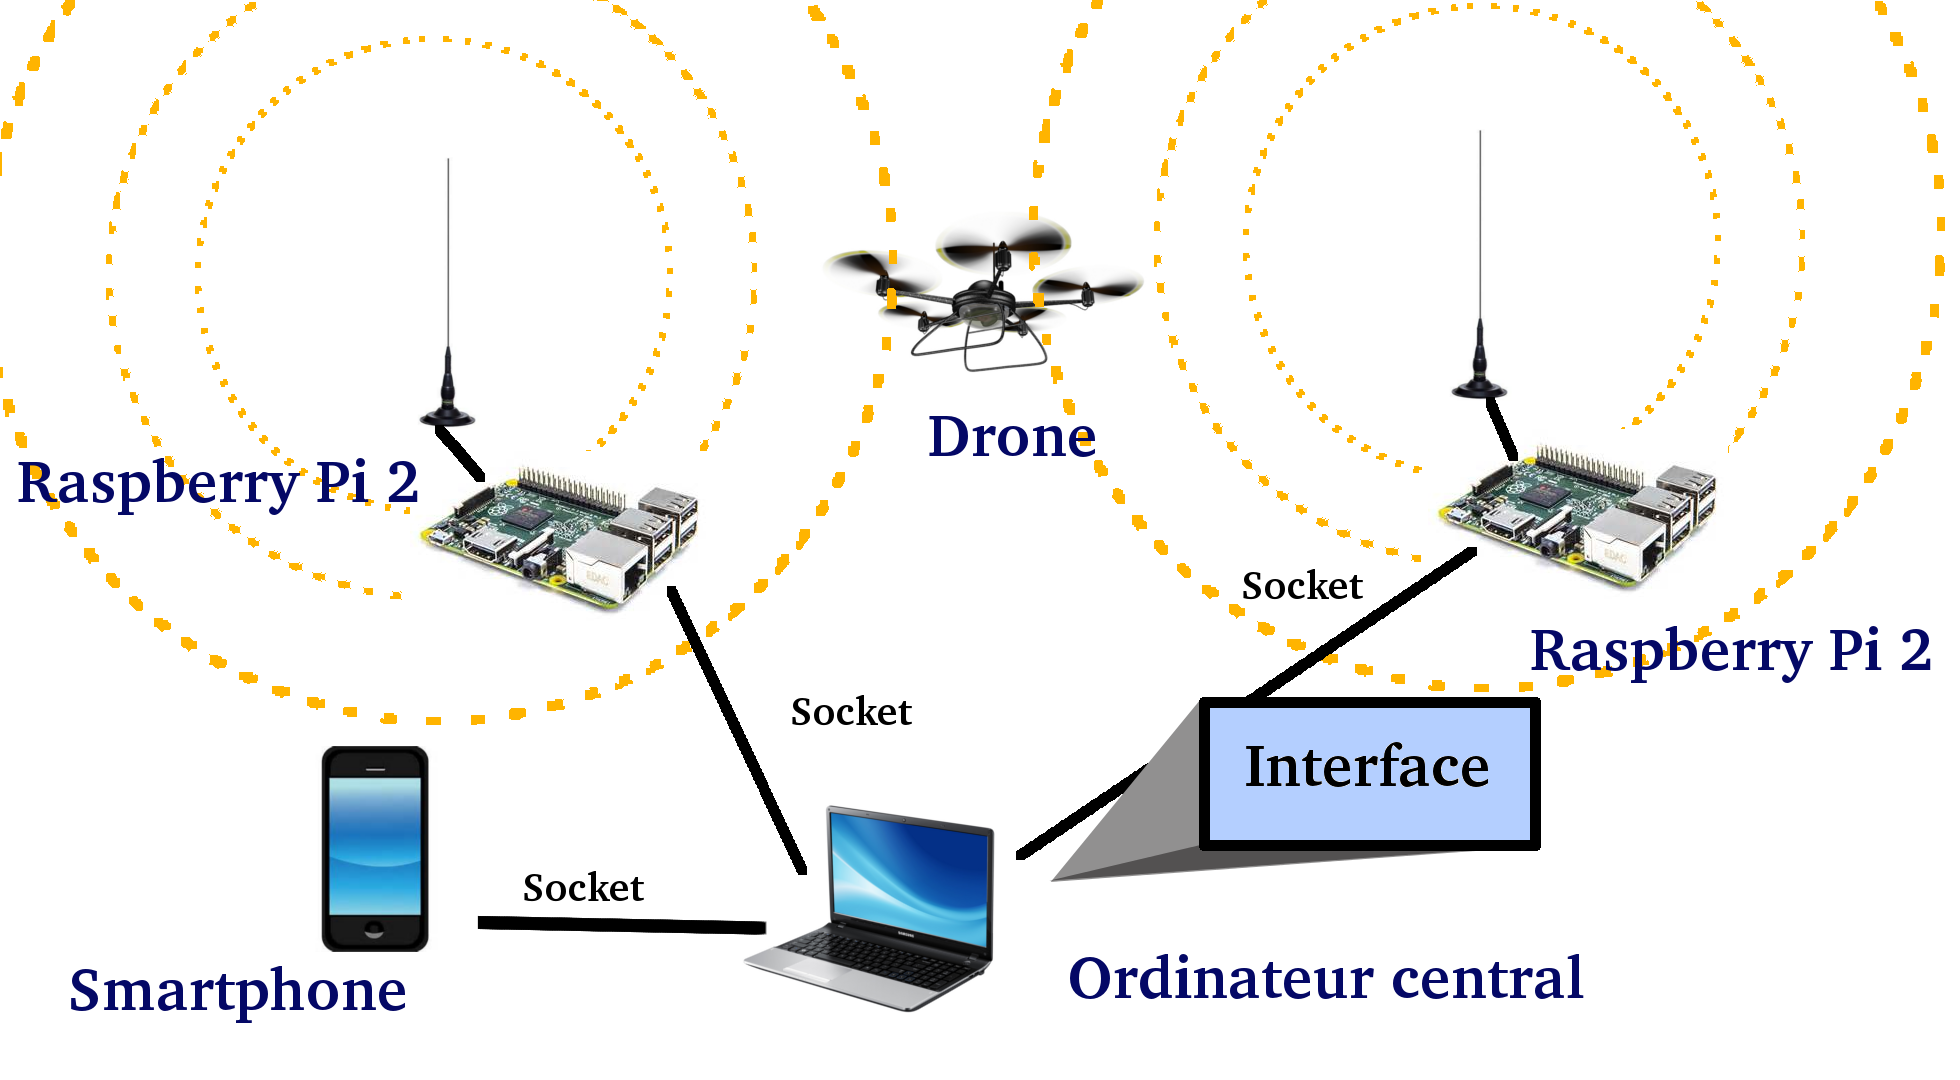
\includegraphics[width=\textwidth]{installation}
  \caption{Installation de Smart}
  \label{fig:inst}
\end{figure}


\section{Architecture Fonctionnelle}

\section{Architecture physique}


L'architecture physique du système est présenté à la figure \ref{fig:arch_phys}.

\begin{figure}[!h]
  \centering
  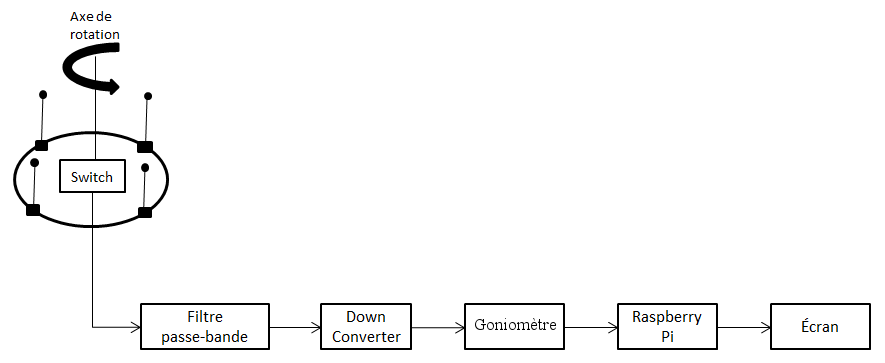
\includegraphics[width=\textwidth]{fonctionnement}
  \caption{Architecture Physique}
  \label{fig:arch_phys}
\end{figure}

\newpage
\section{Treillis de détection}

Pour répondre au besoin de détection et s’assurer d’un correct positionnement de la cible, la mise en
place d’une couverture de détection répondant à nos besoins était nécessaire. Les critères retenus
pour cette dernière sont les suivants :

\begin{itemize}
\item A l’intérieur de la zone de détection, la cible doit être en permanence sous la couverture de détection de 4 radiogoniomètres
\item Tenter une optimisation de la couverture afin d’éviter l’installation d’un trop grand
nombre de radiogoniomètre
\end{itemize}

Très peu de sujets similaires ont pu être trouvé bien que le problème soit récurrent dans de
nombreux projets.

Cependant, après plusieurs essais, le choix de treillis fut le suivant :

\begin{minipage}{0.45\linewidth}

  \centering
  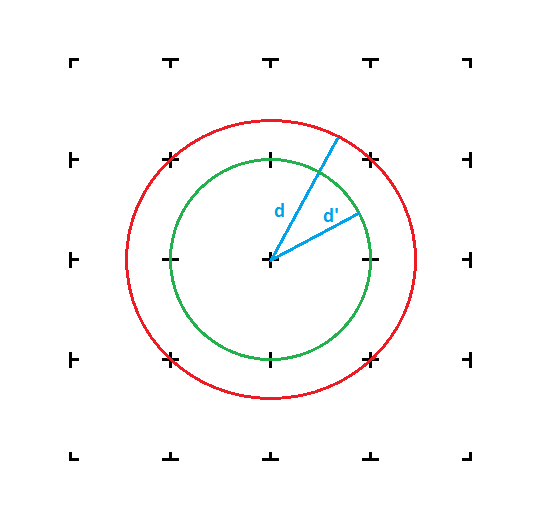
\includegraphics[width=\textwidth]{treillis_explication}
  \captionof{figure}{Cercle de détection}
  ~\\
\end{minipage}
\begin{minipage}{0.45\linewidth}
  \begin{itemize}
  \item Dans les deux cas, les distances d et d’ représente la distance de couverture maximale d’une antenne pour une configuration de treillis particulière, distance au-delà de laquelle nous ne sommes pas sûr d’assurer la détection d’un drone.
  \item Chaque croix noire représente une antenne. Ces dernières formes ainsi la zone de détection, zone à l’intérieure de laquelle, le drone se doit d’être repéré.
  \end{itemize}
\end{minipage}


Initialement, nous avions prévu que les antennes radiogoniométrique assureraient la détection
jusqu’à son plus proche voisin. Cependant, cette configuration ne permet pas d’assurer qu’un drone
traversant la zone soit sous la couverture d’au moins quatre antennes en tout temps. Nous avons
donc choisi la configuration représentée par le cercle rouge, c’est-à-dire en rapprochant les antennes
les unes des autres. On obtient ainsi la couverture suivante :
~\\

\begin{minipage}{0.45\linewidth}
  \centering
  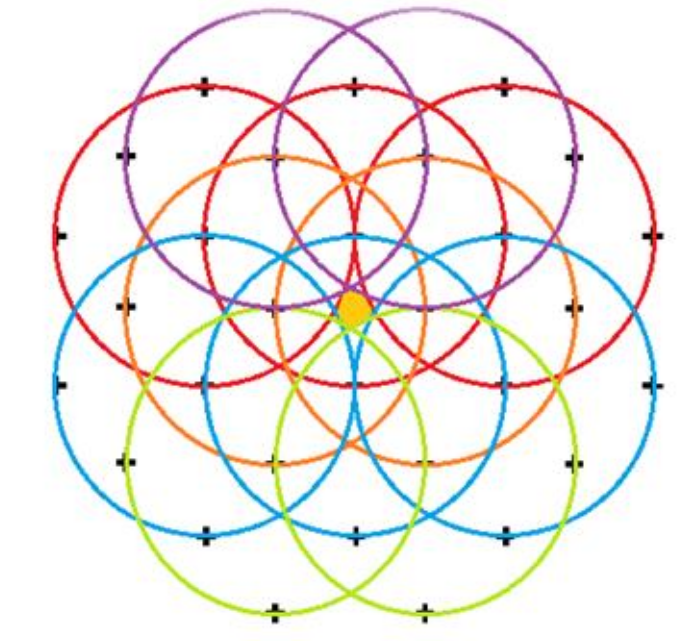
\includegraphics[width=\textwidth]{cercle}
  \captionof{figure}{Maillage de détection}
\end{minipage}
\begin{minipage}{0.45\linewidth}
  Dans cette configuration, les zones de plus faible couverture
sont situées sur les antennes elles même. En effet, au-dessus
de chaque antenne, la couverture n’est assurée que par
quatre d’entre elles. En dehors de celle-ci, la couverture est
assurée par cinq à six antennes.
\end{minipage}




%%% Local Variables: 
%%% mode: latex
%%% TeX-master: "../rapport"
%%% End: 
